\section{Combining Source Code Analysis with Information Privacy Risk Assessment}

\mH apps have been examined in various research studies that aim at providing insights for developers as well as for users into how private information is processed.
Privacy issues are the most impactful user complaints while using mobile apps.\footnote{See \cite{Khalid2015}, p. 5.}
Especially \mH apps deal with sensitive and vulnerable user information and therefore pose a high information privacy risk. \footnote{See \cite{Kumar2013}, p. 33.}
This encourages research to address information privacy risks.

\subsection{Information Privacy Risk Assessment}

% Definition IPR
Information privacy can be defined as the circumstance that people are able to control if, how and where information and knowledge about themselves is acquired, stored and processed.\footnote{See \cite{Fischer1998}, p. 421-422.}
In addition to mere control over the users private information, society and social structure must establish an information regulation architecture that allows people to sustainably enforce their information privacy rights.\footnote{See \cite{Solove2002}, p. 1115.}
An information privacy risk is therefore, by implication, a threat or a circumstance that disables users to enforce control over their private information.
Threats to information privacy in digital services can happen at application level (e.g. by sharing users' personal information with third-parties), as well as at communication level (e.g. by using an unencrypted data connection).\footnote{See \cite{Fischer1998}, p. 423-427.}

% mHealth context
For this thesis, we chose the context of \mH apps, since \mH are commonly handling sensitive user information and are therefore more prone to information privacy violations.\footnote{See \cite{Huckvale2015}, p.1-2.}
Research in the field of information privacy risk assessment of \mH apps has progressed, but research literature in this field is still behind its full potential.\footnote{\cite{Arora2014}, p. 143.}

Information privacy risk classification frameworks were developed to structure the problem of information privacy violation into risk types.\footnote{See for this paragraph\cite{Lewis2014}, p. 2-3.}
Risk types can range from \textit{loss of reputation}, where a \mH apps for instance display sensitive data to unauthorized viewers up to \textit{Inappropriate and irreversible clinical action}. 
The latter type would be reached by a defective algorithm within a \mH app that proposes wrong information.

Even though classifications of information privacy risks exist\footnote{See \cite{Lewis2014}, p. 1-3.} and subsequent regulations and policies have been put in place, \mH apps might not follow these regulations.\footnote{See \cite{Huckvale2015}, p. 1-2.}
A way to identify those apps, that claim to follow common regulations and policies, but secretly still collect sensitive information in inappropriate manners, is by applying special technology to the identification process.\footnote{See \cite{Huckvale2015}, p. 1-2, \cite{Arora2014}, p. 149.}

% Technical side
Research focus has been put on the technical side of information privacy violations and threats. 
It is possible to analyze the Android log files that \mH app might write data into as well as \acl{HTTP} (\acs{HTTP}) data connections to internet servers.\footnote{See \cite{Huckvale2015}, p. 2-5.}

It has been analyzed, to what degree the data storage in internal Android log files or on the memory card within a phone or tablet as well as data connections to the Internet pose threats to users information privacy.\footnote{For this and the next sentence, see \cite{He2014}, p. 645-646, 649.}
Special focus has been put on unencrypted HTTP connections that send out user information to either the app providers servers or third party services.
The assessment has been carried out using the network analysis tool \textit{Wireshark}\footnote{\url{https://web.archive.org/web/20160710141347/https://www.wireshark.org/}, visited 07/13/16.} that logs all HTTP traffic.\footnote{See \cite{He2014}, p. 649.}
Technical evaluation of mobile apps goes further, into the topics of decompilation to analyze device identification or geolocation data leaks.\footnote{See \cite{Mcclurg2012}, p. 1, 5., \cite{Enck2011}, p. 1. and \cite{Mitchell2013}, p. 6-7.}
In conclusion, decompilation is a widely used assessment technique for \ipr and data leaks.

\subsection{Static Code Analysis}

As suggested in previous research, insights from other fields of study can be used to elaborate on the assessment of information privacy risks in the \mH sector.\footnote{See \cite{Arora2014}, p. 143.}

The informatics and software development sector bears tools that could be applied to \ipr assessments of \mH apps.
One of these tools is a static code analysis.
Static code analysis refers to analysing the source code of a software without actually executing the software.\footnote{See \cite{Louridas2006}, p. 58.}

In informatics and software development contexts, \sca has been used to analyze source code\footnote{See \cite{Haris2014}, p.  5.} and provide feedback on coding styles to the users while programming\footnote{See \cite{Bardas2010}, p. 10.} or to identify fault in software source code\footnote{\cite{Bardas2010}, p. 1.}.\footnote{This paragraph follows \cite{Louridas2006}, p. 58.}
\Sca provides a fast way to analyze source code\footnote{See \cite{Bardas2010}, p. 5.}, which makes it suitable to automate the assessment of large amounts of data.
A further benefit of using \sca to retrieve information from software is that the software does not need to be executed during the analysis process.
This additionally supports the development of fast performing assessment tools that are suitable for application on large datasets of source code.
There is no need to wait for the application runtime to execute the software in performing a static code analysis.

In the context of \mH apps, the analysis of data connection using software that intercepts the HTTP traffic of the \mH to internet servers has been performed.\footnote{See \cite{Mense2015}, p. 42.}
The results of the HTTP traffic anlysis show that information privacy leaks via unencrypted internet connections are common.\footnote{See \cite{Mense2015}, p. 42-44.}

Static code analysis is also used as an intermediate step in achieving an \ipr analysis, in previous research.\footnote{For this and the following sentence, see \cite{Dorazio2015}, p. 5177, 5179-5180.}
The \sca step within the aforementioned analysis process is performed manually by a human researcher and not part of an automated process.
It is therefore only applicable for small amounts of apps to be reviewed at a time.

\textcite{Knorr2015} propose the idea to automate the information privacy risk analysis further, in future research.\footnote{For this and the following sentence, see \cite{Knorr2015}, p. 1.}
The \sca in the case of the study by \textcite{Knorr2015} uses a multitude of software tools to perform the analysis of only 9 attack scenarios.

Our study will use the benefits of \sca and apply them to the assessment of \mH information privacy risks.
It is yet unclear if \sca is a viable tool to automatically analyze and identify information privacy risk factors.
We will use the comprehensive information privacy practices that \cite{Dehling2016} identified\footnote{See \cite{Dehling2016}, p. 8-17.} and try to implement \sca strategies to identify the information privacy practices that bear risks, automatically.
This will be a vital addition to current research, since there is yet no holistic approach to apply and no automated \sca to \ipr detection that takes an adequate amount of \iprfs into account.

\subsection{Relevant Information Privacy Risk Factors}\label{chapter:Relevant}

For this thesis, we will use the set of \ipp extracted from literature, the Platform for Privacy Preferences (\acs{P3P}) guide\footnote{\url{https://web.archive.org/web/20160616160213/http://www.w3.org/TR/P3P/}, visited 06/16/2016.} and app reviews by \cite{Dehling2016} as sources to derive \iprfs from.\footnote{For this and the following sentence, see \cite{Dehling2016}, p. 1-2.} 
\Ipp are common content aspects and practices of informing users about the information privacy practices of an app. 
App providers should follow these \ipp in order to achieve higher levels of transparency.
A hierarchy of \ipp is formed by clustering the information privacy practices. 

\begin{figure}[h]
	\centering
	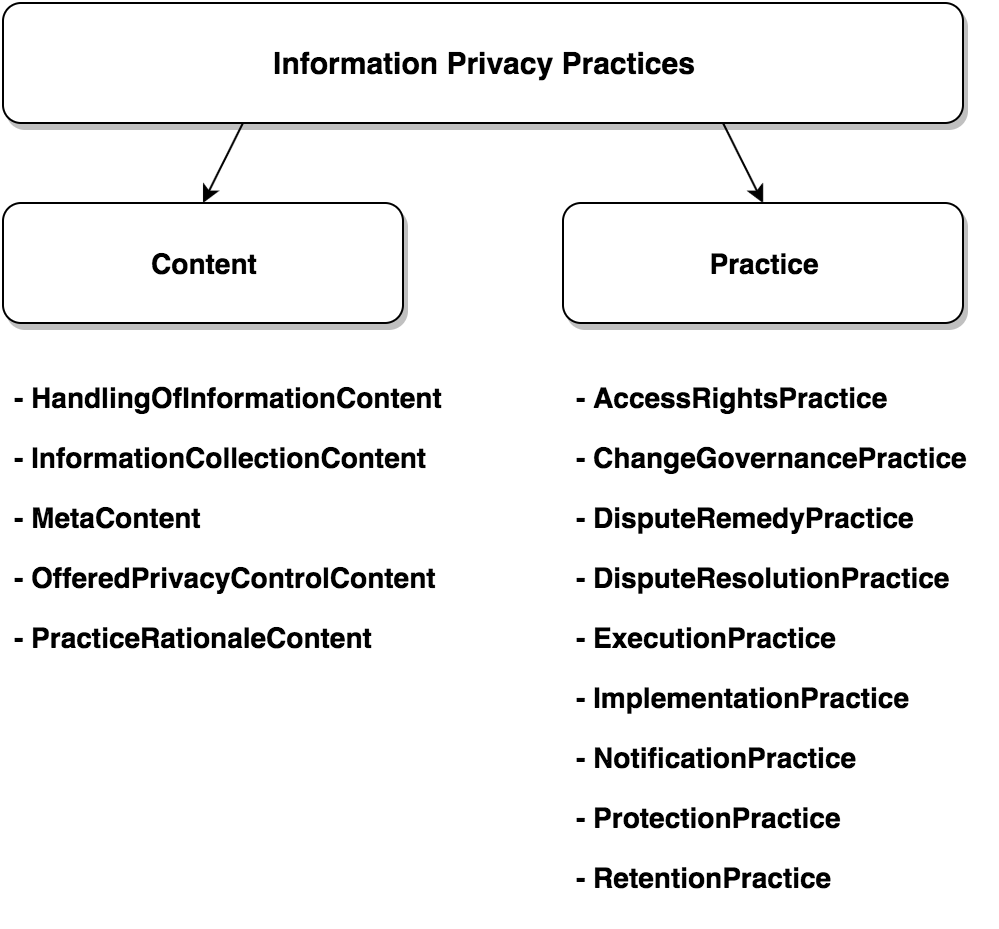
\includegraphics[keepaspectratio=true,width=350pt]{figures/IPP.png}
	\caption{Diagram of the hierarchy of information privacy practices, proposed by \cite{Dehling2016}.}
	\label{fig:informationPrivacyPractices}
\end{figure}

The top levels of the hierarchy, as seen in figure \ref{fig:informationPrivacyPractices}, are \textit{Content} and \textit{Practice}.
The \textit{Content} hierarchy level contains sub-hierarchy branches that express \ipp concerning the handling of information content, the information collection content, and meta content about information collection, information on offered privacy controls, and information on what purpose the \ipp were collected for.

We argue, if an information privacy practice is a circumstance that the user should be informed about, an information privacy practice expresses an information privacy risk to the app user.
But since not all of the enlisted \ipp express or imply an information privacy risk to app users, we review and extract the \ipp that are relevant in terms of posing and expressing a potential information privacy risk.
The classification of \ipp that bear or express an information privacy risk will be conducted by two researchers separately.
The results of the two researchers will be discussed to find common consensus about the classification.
We will further limit the \ipp by excluding \ipp that are known to be technically infeasible to detect via static code analysis of the app source code.
An example for such an exclusion is the information privacy practice \textit{InformationRetentionContent}, which captures, if an app provider carries out a certain information retention policy or not.\footnote{See \cite{Dehling2016}, p. 8.}
This is a feature that is undetectable by \sca and beyond the scope of app source code analysis.
An analysis of the app providers backend system would be necessary to ensure that the collection information is retained according to the app providers policy promise.

We include a full list of all \ipp in Appendix A including detailed comments on the technical limitations, if any, towards the \sca detection of each \ipp and wether they express a risk or not.

The following \ipp were identified as relevant to the \sca and further inspection within this thesis:

The complete hierarchy \textit{CH2} 'InformationSecurityContent' can be analysed via \sca including the \ipp 'SecurityDuringProcessingContent', 'SecurityDuringStorageContent' and 'SecurityDuringTransferContent'.
Partially supported will be the hierarchy \textit{CH3} 'InformationSharingContent'. Analysis will be applied to the containing \ipp \textit{CH33} 'SharingWithAdvertiserContent', \textit{CH34} 'SharingWithAggregatorContent', \textit{CH35} 'SharingWithAnalystContent', \textit{CH36} 'SharingWithDeliveryContent', \textit{CH37} 'SharingWithGovernmentContent', \textit{CH38} 'SharingWithOtherUsersContent', \textit{CH310}, \textit{CH311} 'SharingWithUnrelatedContent' 'SharingWithPublicContent' and \textit{CH312} 'SharingWithUserAuthorizedContent'.
The hierarchy \textit{CH4} 'InformationStorageContent' is relevant and can be analysed via static code analysis, as well as the hierarchies \textit{CI21} 'EnvironmentSensorContent', \textit{CI22} 'LocationSensorContent', \textit{CI23} 'UserSensorContent' and all their coherent sub-hierarchies.
For the hierarchy \textit{CI24} 'SoftwareUseSensorContent' only partial support for the sub-hierarchies \textit{CI242} 'CookiesContent' and \textit{CI243} 'SurveysContent' are feasible to be analyzed by static code analysis.
With the exception of one \ipp in the hierarchy level \textit{CI31} 'InformationFormContent' all other \ipp are relevant for this thesis: \textit{CI311} 'AudioInformationContent', \textit{CI312} 'ImageInformationContent', \textit{CI314} 'TextInformationContent' and \textit{CI315} 'VideoInformationContent'.
The next hierarchy level \textit{CI32} 'IdentifierContent' is fully relevant and all coherent sub-hierarchies will be analyzed.
More difficult to analyze via \sca will be the hierarchy level \textit{CI33} 'OperationalContent', because only two \ipp were identified as relevant to static code analysis: \textit{CI333} 'LocationContent', \textit{CI335} 'OnlineContactsContent' and \textit{CI336} 'PurchasesContent'.
Finally the hierarchy \textit{CI34} 'UserDetailsContent' is partially relevant, namely the \ipp \textit{I341} 'DemographicsContent', \textit{CI343} 'HealthContent', \textit{CI344} 'IdeologicalContent', \textit{CI345} 'PreferencesContent' and \textit{CI346} 'UserDeviceContent'.

All relevant \ipp and their \sca identification strategies will be explained further in chapter \ref{sssec:SCAP} of this thesis.
